\documentclass[11pt, twoside, hidelinks, letterpaper,openany]{book} 
\usepackage[english]{babel}
\usepackage[utf8]{inputenc}
\usepackage[T1]{fontenc}
\usepackage[margin = 3cm, vmargin=2.5cm,includefoot]{geometry} 
\usepackage{wrapfig}
\usepackage{pgfgantt} % grant diagrams
\usepackage{float} %images
\usepackage{amsmath} %Greek letters 
\usepackage{siunitx} %scientific notation
\usepackage{enumitem} %descriptive list
\usepackage{caption} % for figure
\usepackage{subcaption}%for sub figure
\usepackage{titlesec} %title style
\usepackage{fancyhdr} % Page style
\usepackage{lipsum} %random \lipsum text
\usepackage{ragged2e} %Alignment and  justification
\usepackage{pdflscape} %sheet orientation
\usepackage{booktabs, multicol, multirow, longtable, colortbl, xcolor, tabularray} %Tables
\definecolor{Gray}{gray}{0.85}
\usepackage[table]{xcolor}
\newcolumntype{s}{>{\columncolor{Gray}} p{0.1\textwidth}}
\usepackage{array}
\usepackage{csquotes} 
\usepackage{url}
\usepackage[bottom]{footmisc} %Images bellow footer
\usepackage{pdfpages}
\usepackage{attachfile2}

%-----------------------------------------------------------------------
% images
\usepackage{graphicx}
%\usepackage{subfig}
\usepackage{epstopdf}
\usepackage[lighttt]{lmodern}
\usepackage{listings}
\DeclareGraphicsExtensions{.svg, .png,.pdf, } %image search order

%-----------------------------------------------------------------------
% Page format
\pagestyle{fancy} %style of Page
\fancyhf{} %clean header and footer
\cfoot{\thepage} %footer at right
\renewcommand{\headrulewidth}{0pt} 
\renewcommand{\footrulewidth}{0pt} 

%-----------------------------------------------------------------------
%Bibliography
\usepackage[
    backend=biber,
    block=space,
    dashed=false,
    uniquelist=false,
    mincitenames=1,
    maxcitenames=3,
    style=ieee]{biblatex} 
    %https://da.sharelatex.com/learn/Biblatex_bibliography_styles
\addbibresource{references.bib} %bib file
\NewBibliographyString{teststring}
\NewBibliographyString{andothers}
\DefineBibliographyStrings{english}{
  teststring = {Test string},
  andothers = {et\addabbrvspace al\adddot}
}
\usepackage{hyperref} 

\AtEveryBibitem{
\ifentrytype{misc}
    {}
    {\clearfield{url}} 
}
% ----------------------------------------------------------------------

\graphicspath{{images/}}


\titleformat{\section}
{\centering\bfseries}  
{\thesection}  
{1em} 
{}  

\titleformat{\subsubsection}
{\bfseries}
{\thesubsubsection}
{1em}
{}

\setcounter{secnumdepth}{3} %Sections depth
\setcounter{tocdepth}{3} %Sections depth in table of contents



%-----------------------------------------------------------------------


\begin{document}

\frontmatter
\graphicspath{{images/}}
\begin{titlepage}

    \begin{center}
        \hspace*{1cm}
        
        \begin{figure}[H]  
         \centering
         
\includegraphics[width=0.3\textwidth, height=0.3\textwidth]{logo-umng.png} 
        \end{figure}            
        
        \large
        \textbf{Development and implementation of a parallel ankle rehabilitation robot: PRANK } 

        % - PRANK: Development of a Parallel Robot for ANKle Rehabilitation Using Admittance Control and Virtual Reality
        % - Design and Implementation of PRANK: A Parallel Robot for ANKle Rehabilitation with Adaptive VR-Based Therapy
        % - PRANK—A Parallel Ankle Rehabilitation Robot with Force Feedback and Serious Game Integration
        % - Development and Validation of PRANK: A Parallel Robotic Platform for Ankle Rehabilitation Using ROM and Force-Adaptive Control
        % - PRANK: A Mechatronic System for Ankle Rehabilitation through Parallel Robotics and VR Feedback
%


        \vspace{3cm}
        
        \large
        \textbf{Ante-project presented by: \\Luis Fernando Salamanca Sánchez}
        
        \vspace{2cm}
        \vspace{2cm}
        
        \textbf{Supervised by:}\\
        \textbf{Ruben }\\
        
        \vfill
        
        
        
        
        UNIVERSIDAD MILITAR NUEVA GRANADA \\
        MASTER'S DEGREE PROGRAM IN MECHATRONICS ENGINEERING. \\
        BOGOTÁ D.C \\
        2025
    \end{center}
\end{titlepage}
\setcounter{page}{1}
\thispagestyle{fancy}

\section*{PROPOSAL SUMMARY SHEET}
\phantomsection
\addcontentsline{toc}{section}{\numberline{}Acknowledgments}

\begin{enumerate}
    \item Date of submission of grade option: 25/04/2025
    \item Summary table
    \begin{table}[h]
        \centering
        \begin{tabular}{|s|m{0.8\textwidth}|}
        \hline
          Title   &  Development and implementation of a parallel ankle rehabilitation robot: PRANK \\
        \hline
          Area   & Robotics  
          \\
        \hline
          Research Group & DAVINCI  
          \\
        \hline
          Type of research & Experimental development
          \\
        \hline
        \end{tabular}
        \caption{Proposal Summary Table}
        \label{tab:summary}
    \end{table}
    \item Author data:
    \begin{table}[h]
        \centering
        \begin{tabular}{|c|c|c|}
        \hline
        \rowcolor{Gray}
            \textbf{Student Code} & \textbf{Name} & \textbf{ID}\\
        \hline
            3900317 & Luis Fernando Salamanca Sánchez & 1002460999\\
        \hline
        \rowcolor{Gray}
            \textbf{Phone} & \textbf{E-mail}  \\
        \cline{1-2}
            +573508501607 & est.luisf.salamanca@unimilitar.edu.co\\
        \cline{1-2}
        \end{tabular}     
        \caption{Author data}
        \label{tab:author_data}
    \end{table}
\end{enumerate}

%\null \vspace{\fill}

\section*{Abstract}
\phantomsection
\addcontentsline{toc}{section}{\numberline{}Abstract}
\graphicspath{{images/}}


Human gait is a fundamental component of mobility, autonomy, and overall quality of life. Among the joints involved in locomotion, the ankle plays a crucial role in absorbing shock during heel strike and facilitating propulsion during the push-off phase. Impairments in ankle function—whether due to neurological conditions, trauma, or post-surgical recovery—can significantly compromise gait, balance, and independence. Robotic rehabilitation has emerged as a promising alternative to traditional therapy, offering consistent, repeatable, and quantitatively measurable support.

This project proposes the development of a Parallel Ankle Rehabilitation Robot (PARR), actuated through an RRR electric motor configuration and controlled via an admittance algorithm based on real-time force feedback. The system is complemented by a serious game implemented in virtual reality, designed to enhance patient engagement and tailor therapy difficulty dynamically based on ankle range of motion (ROM) and user-applied force. The project focuses on the mechatronic development of the robot and the comparative validation of its ROM measurement accuracy against an optoelectronic motion capture system, aiming to demonstrate the system’s feasibility for reliable biomechanical evaluation and future deployment in clinical environments.

esto es una prueba que estoy viendo si el live editor funciona


\tableofcontents
\listoffigures
\listoftables
\addtocontents{toc}{\protect\thispagestyle{empty}} 
\let\cleardoublepage\clearpage %Delete footer after index


\mainmatter
\include{Chapters/problem_statement}
\chapter{PROJECT JUSTIFICATION} \label{results}
\graphicspath{{images/}}

Gait is a fundamental aspect of human independence and well-being. Within the gait kinetics, the ankle joint plays a pivotal role in absorbing impact forces during heel strike and generating propulsion during toe-off. When the ankle's function is impaired—due to conditions such as stroke, orthopedic trauma, or neurodegenerative disease—patients face significant limitations in mobility, balance, and daily autonomy.

Rehabilitation is essential for restoring ankle functionality, yet conventional methods often lack the consistency, objectivity, and sustained engagement required for optimal recovery. Furthermore, existing robotic devices for gait rehabilitation typically do not include mechanisms specifically designed for targeted ankle strength recovery. In this context, robotic rehabilitation systems offer the advantages of repeatability, precise measurement, and the ability to adapt therapy to an individual’s progress. Additionally, serious games and virtual reality environments have shown considerable promise in enhancing motivation and participation—key factors that directly influence rehabilitation outcomes.

This project addresses these needs through the development of PRANK (Parallel Robot for ANKle rehabilitation), a parallel robotic platform actuated by an RRR configuration and controlled through admittance strategies. It aims to offer a safe, adaptive, and engaging therapeutic environment. By integrating a serious game and a real-time feedback loop that adjusts difficulty based on force and range of motion (ROM), the system seeks to promote user-centered recovery while providing measurable, high-fidelity data. Additionally, validating PRANK’s ROM measurement capabilities against an optoelectronic motion capture system will support its use as a reliable biomechanical assessment tool in future clinical settings.
\chapter{STATE OF ART}\label{state_art}
\graphicspath{{images/}}


\chapter{OBJECTIVES}

\section{General}

Develop a parallel ankle rehabilitation robot using admittance control strategies, serious virtual reality-based games and an RRR electric motor configuration, adapting the difficulty of therapy based on real-time ankle range of motion (ROM) and force feedback.

\section{Specifics}
\begin{itemize}
    \item Design, fabricate and assemble a 3-axis parallel structure based on electric motors to fit the controlled movement of the ankle.
    \item Develop an admittance control system that adjusts therapy resistance based on patient interaction, based on force feedback, ensuring adaptive rehabilitation.
    \item Create a virtual reality serious game to engage patients in interactive rehabilitation, enhancing motivation and adherence to therapy.
    \item Implement a difficulty adjustment algorithm based on real-time ankle ROM measurements to provide progressive rehabilitation tailored to the patient's recovery status.
    \item Evaluate system performance through simulations and subject trials, measuring effectiveness in improving ankle mobility, patient experience, ROM calculus and control algorithm performance. 

\end{itemize}
     
    
\chapter{DELIMITATION AND SCOPE}\label{delimitation_scope}
\graphicspath{{images/}}

This project encompasses the design, development, and initial technical validation of a parallel ankle rehabilitation robot (PARR) featuring an RRR configuration and admittance control. The system integrates real-time force feedback and a virtual reality-based serious game to promote engagement and adaptive therapy based on ankle range of motion (ROM). The scope includes mechanical design, electronic design, control system implementation, development of the VR environment, and a ROM evaluation strategy using an optoelectronic motion capture system as a reference standard.

However, the study is delimited to engineering and software development stages. It does not involve clinical trials with patients or assessment of long-term rehabilitation outcomes. Likewise, while the VR component is designed to enhance engagement, this work does not evaluate its psychological or motivational impact. Validation efforts are limited to simulations and technical comparisons with healthy subjects or artificial inputs to quantify kinematic performance and ROM estimation accuracy.
 
\chapter{HYPOTHESIS}\label{HYPOTHESIS}

The developed parallel ankle rehabilitation robot, controlled via an admittance-based algorithm and integrated with a serious virtual reality game, will be capable of accurately estimating the ankle's range of motion (ROM). The ROM values derived from the system will show strong correlation and minimal deviation when compared to those obtained from a validated optoelectronic motion capture system, thereby demonstrating the feasibility of reliable kinematic assessment through the robot’s onboard sensors and software.
\chapter{THEROTICAL FRAMEWORK}\label{introduction}
\graphicspath{{images/}}

% Importance of ankle in the gait and all the diseases that causes footdrop or similars, and the solutions for this desease.

\section{theoretical framework}\label{framework}

\section{Human gait}

The gait analysis is carried out on the basis of the gait cycle, that can be taken as representation of person's walking patterns, and comparison of several cycles indicates the variability of the pattern \cite{Baker2013}. The gait cycle is normalized from 0\% to 100\%, because each pattern have different timing, so is not objective realize a comparison between them \cite{Medved2021}, it can be described with spatial and temporal parameters. 
% \subsection{Spatial parameters}

% The main spatial parameters are shown in figure \ref{step_stride} and described bellow:

% \begin{itemize}
%     \item Step: the movement of the one foot in front of the other.
%     \item Stride: step of one foot followed by another step for the other. 
%     \item Foot contact: it is considered as the beginning of the gait cycle, in healthy people it is referred to as \textit{heel strike}.  
%     \item Step length: distance traveled for one foot in front of the same part of the other foot.
%     \item Stride length: distance between two consecutive gait cycles.
%     \item Step width: mediolateral separation of the feet, also known as stride width.
% \end{itemize}

% \begin{figure}
%     \centering
%     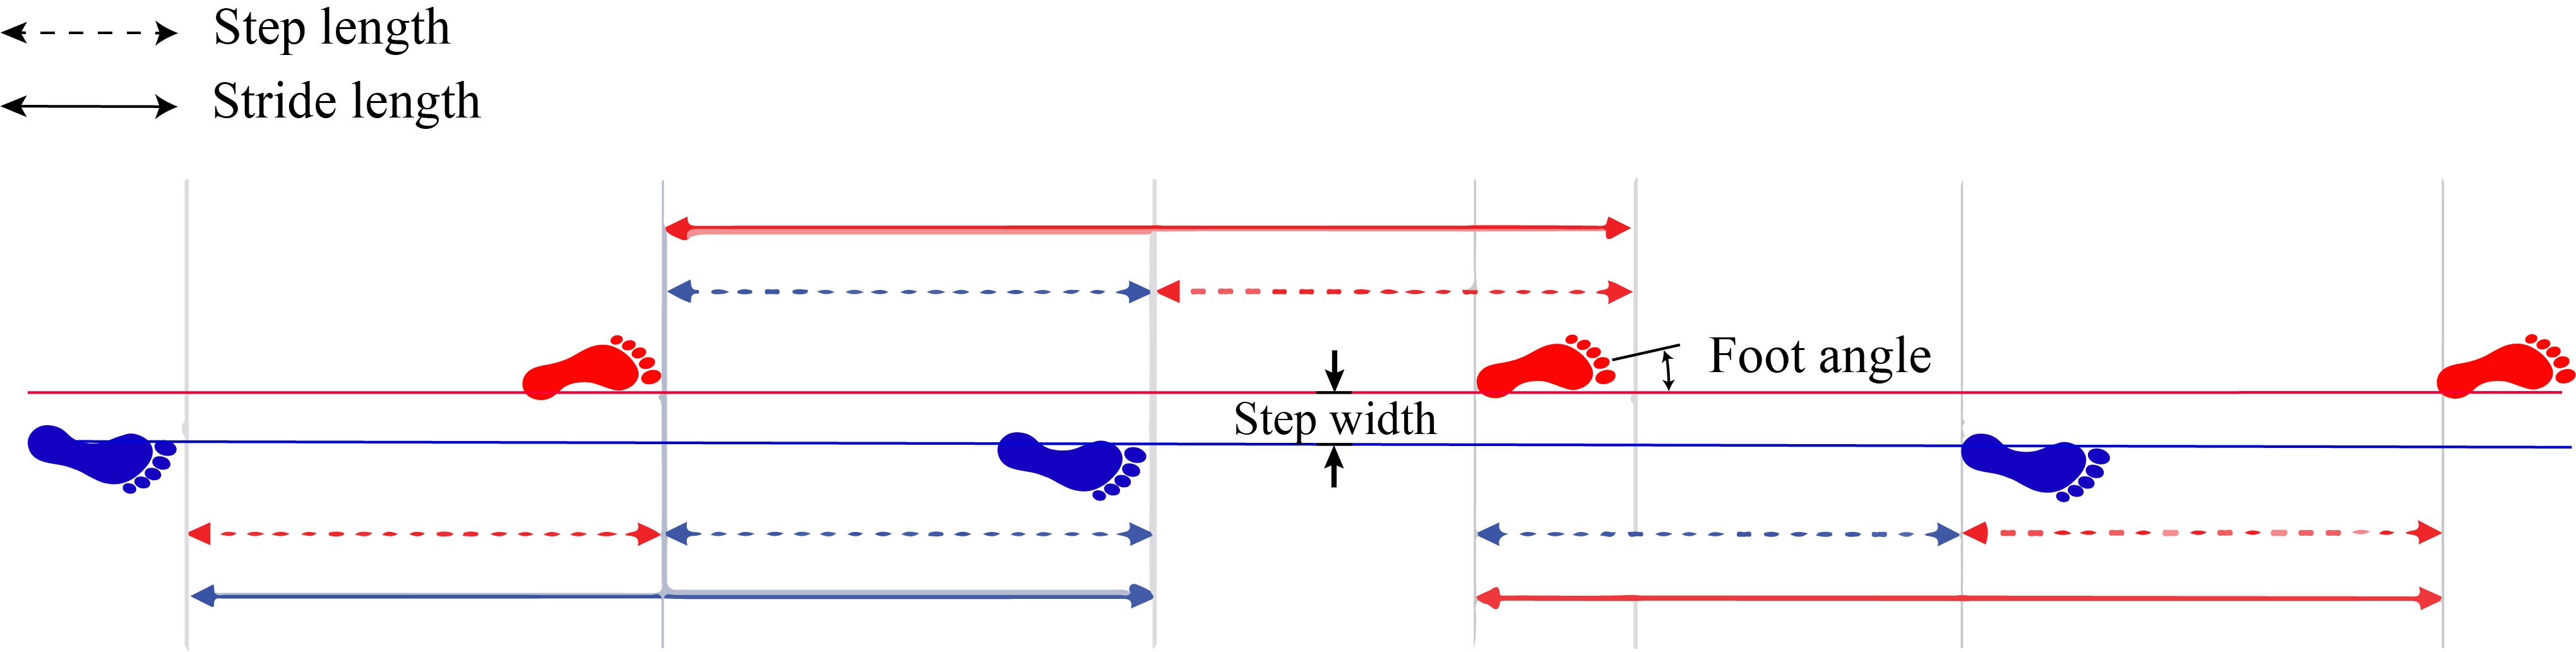
\includegraphics[width=1\textwidth]{step_stride.png}
%     \caption[Gait spatial parameters]{Gait spatial parameters. Source: edited by author from \cite{Baker2013}.}
%     \label{step_stride}
% \end{figure}

% \subsection{Temporal parameters}
% Temporal parameters are listed bellow:

% \begin{itemize}
%     \item Stride time: duration of gait cycle (time between two foot strikes). 
%     \item Cadence: it is a more commonly term used to specify the duration of the cycle in indirect way. And is described by: 
%     \begin{equation}
%         \frac{\#cycles}{time\hspace{1mm}interval}
%     \end{equation}
%     \item Walking speed: distance traveled in a given time in meters/second, if cadence is in steps per minute and stride length is in meters the calculation is given by:
%     \begin{equation}
%         \frac{cadence*stride\hspace{1mm}length}{120}
%     \end{equation}
% \end{itemize}

% Gait is globally divided into two phases, \textit{stance} and \textit{swing}. The first occur when foot is in contact with the ground, on the other hand, the swing occur when it is not. The stance phase ends when foot off (toe off); the same point at which the swing begins, as illustrated in the figure \ref{gait_phases}, 

% \begin{figure}
%     \centering
%     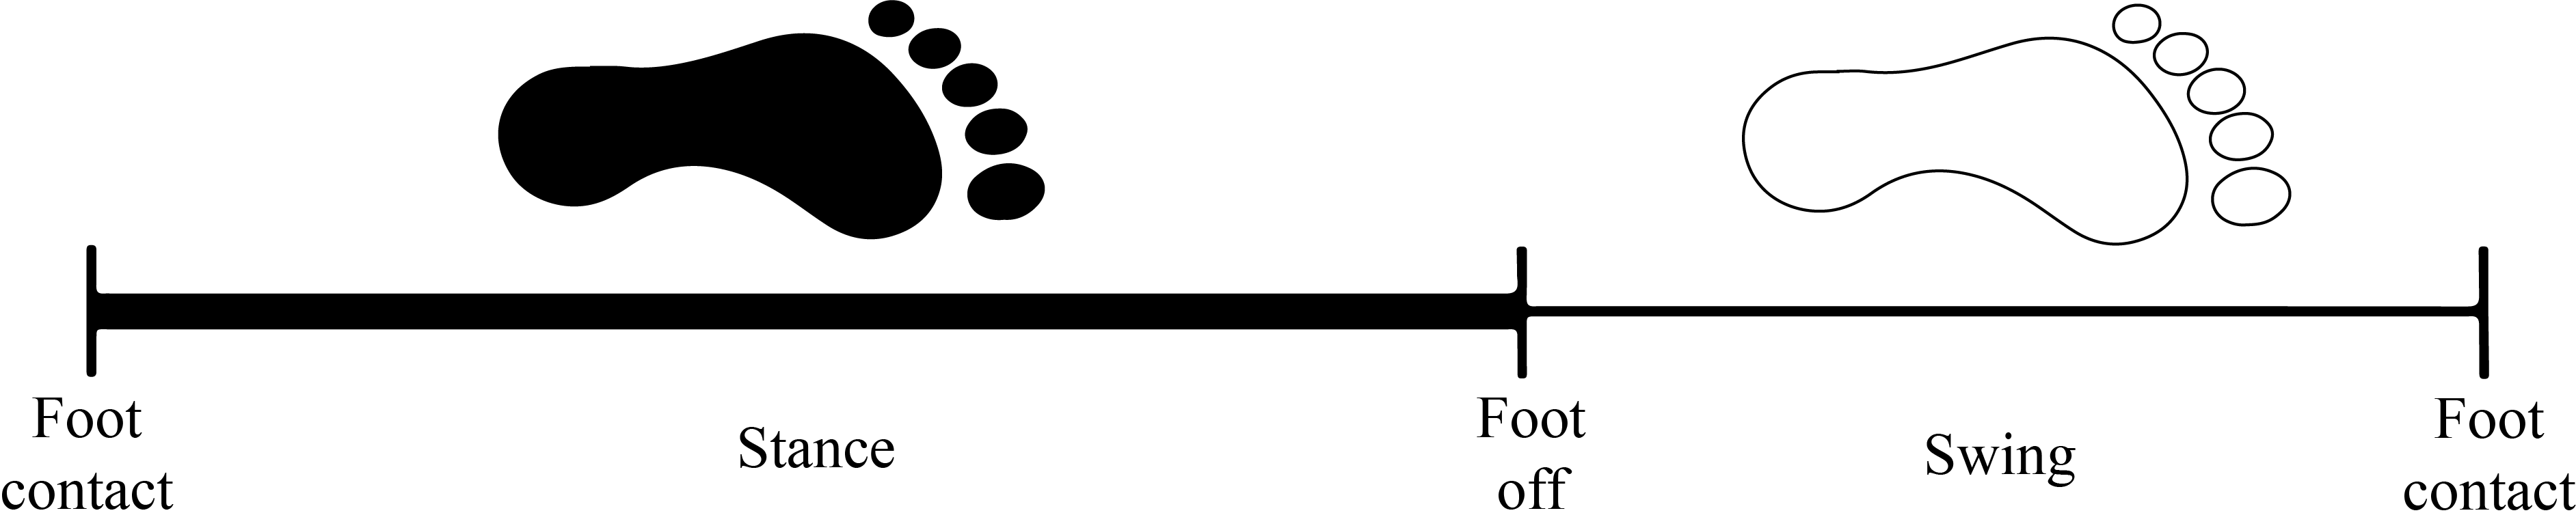
\includegraphics[width=1\textwidth]{gait_phases.png}
%     \caption[One side gait phases]{One side gait phases. Source: edited by author from \cite{Baker2013}.}
%     \label{gait_phases}
% \end{figure}

% The scheme can include the events of both legs, and is divided into first double support (both feet in contact with ground), single support, second double support and swing, as is shown in figure \ref{gait_phases_ds}. Single support and swing are long phases, so a subdivision is a good choice: \textit{early}, \textit{middle} and \textit{late} as can be seen in the figure \cite{Baker2013, Schneck2002}.

% \begin{figure}[b]
%     \centering
%     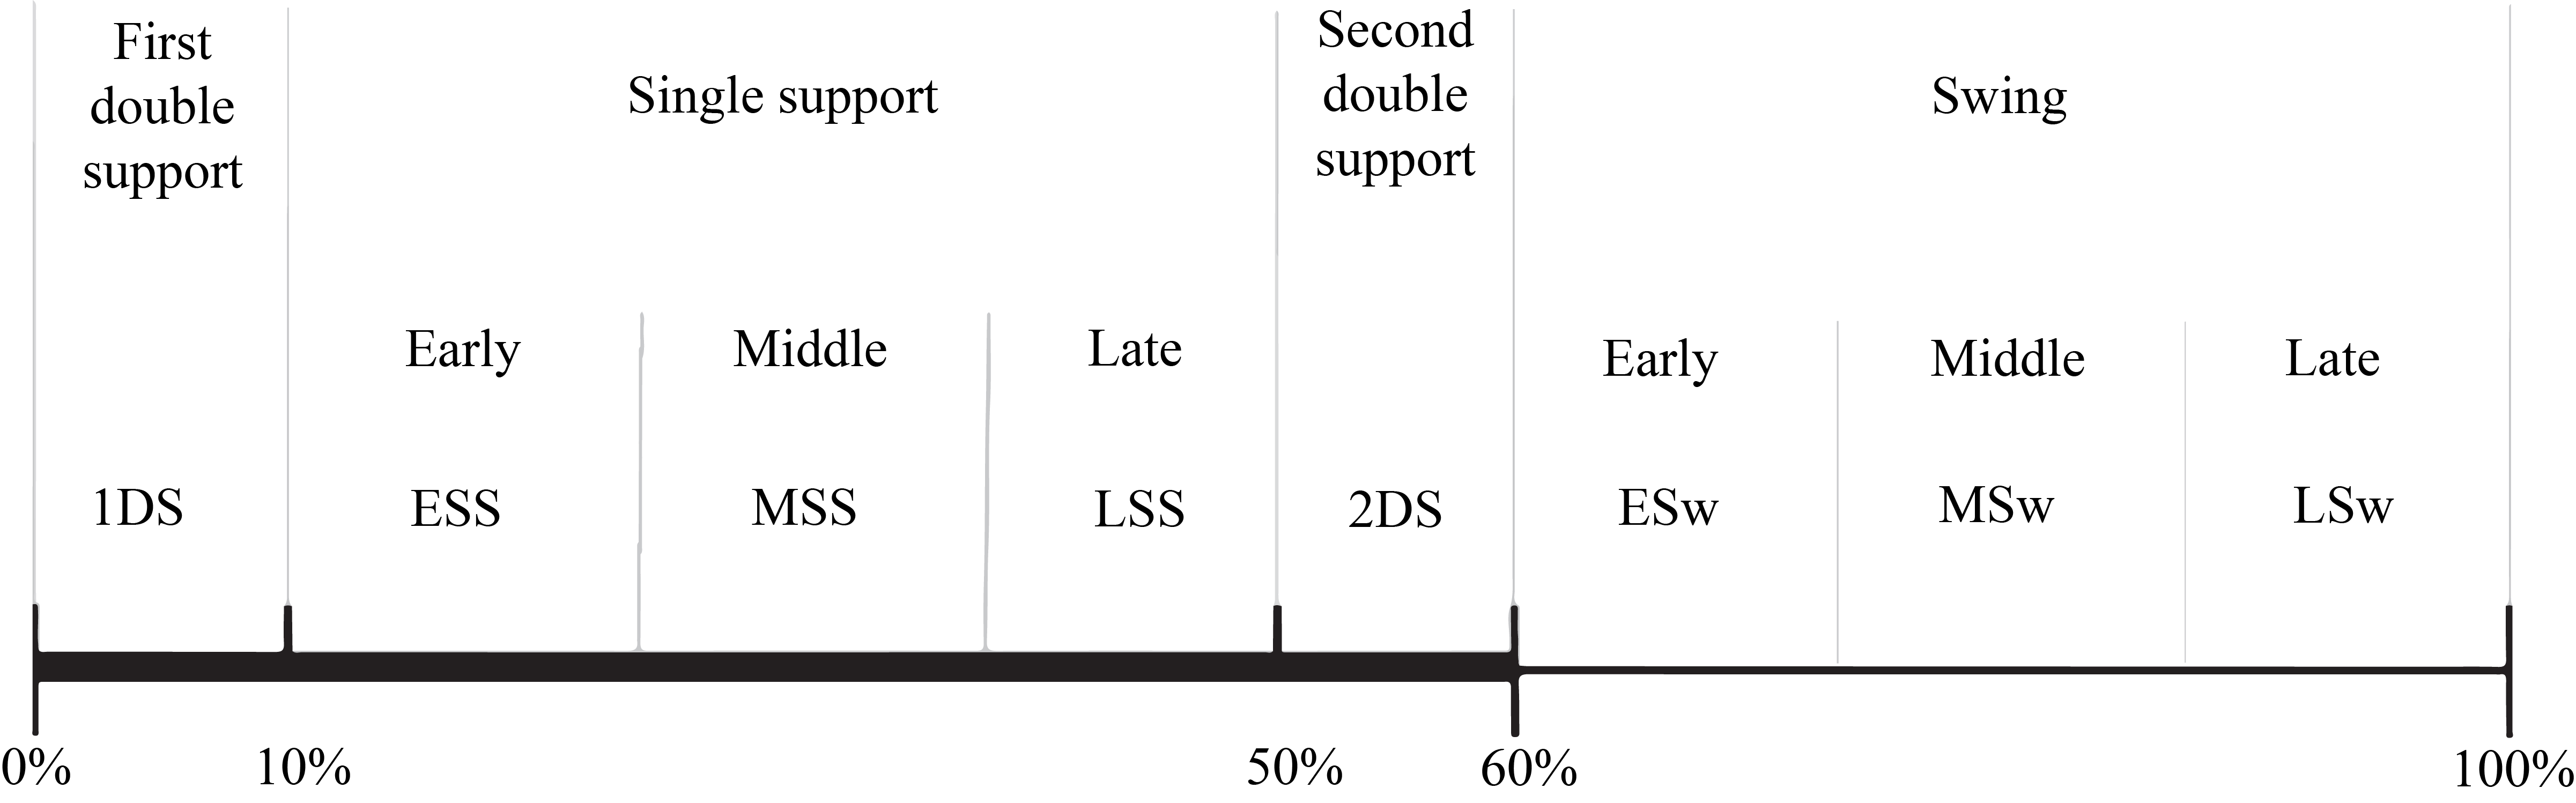
\includegraphics[width=1\textwidth]{gait_phases_ds.png}
%     \caption[Both sides gait phases ]{Both sides gait phases. Source: edited by author from \cite{Baker2013}.}
%     \label{gait_phases_ds}
% \end{figure}
\chapter{MATERIALS AND METHODS}\label{methods}
\graphicspath{{images/}}




\chapter{SCHEDULE}\label{schedule}
\graphicspath{{images/}}

% \begin{figure}[H]
% \centering
% \begin{ganttchart}[
%     hgrid,
%     vgrid,
%     time slot format=is month,
%     bar height=0.6,
%     bar label font=\small\bfseries,
%     x unit=0.65cm,
%     y unit chart=0.9cm,
%     milestone label font=\small\bfseries,
%     milestone height=0.3
% ]{1}{12} % <-- Aquí defines el rango de meses directamente

% % Títulos
% \gantttitle{Project Timeline for PRANK (12 Months)}{12} \\
% \gantttitlelist{1,...,12}{1} \\

% % Tareas
% \ganttbar{Planning and Research}{1}{1} \\
% \ganttbar{Mechanical Design}{2}{3} \\
% \ganttbar{Electronics and Integration}{3}{4} \\
% \ganttbar{Control System Development}{5}{6} \\
% \ganttbar{VR Game Development}{6}{7} \\
% \ganttbar{System Integration}{8}{9} \\
% \ganttbar{Validation and Testing}{9}{10} \\
% \ganttbar{Final Adjustments and Documentation}{11}{12}

% \end{ganttchart}
% \caption{Gantt Chart of Project Tasks for PRANK}
% \label{fig:gantt}
% \end{figure}


\begin{ganttchart}[
    hgrid,
    vgrid,
    bar height=0.6,
    bar label font=\small\bfseries,
    x unit=0.8cm,
    y unit chart=0.9cm,
    milestone label font=\small\bfseries,
    milestone height=0.3,
    bar/.append style={fill=red!50}
     ]{1}{12}
\gantttitle{Project Timeline for PRANK}{12} \\
\gantttitlelist{1,...,12}{1} \\
\ganttbar{Planning and Research}{1}{2} \\
\ganttbar{Mechanical Design}{2}{3} \\
\ganttbar{Electronics and Integration}{3}{4} \\
\ganttbar{Control System Development}{5}{6} \\
\ganttbar{VR Game Development}{6}{7} \\
\ganttbar{System Integration}{8}{9} \\
\ganttbar{Validation and Testing}{9}{10} \\
\ganttbar{Documentation}{1}{12}
% \ganttlinkedbar{Task 2}{3}{7} \ganttnewline
% \ganttmilestone{Milestone}{7} \ganttnewline
% \ganttbar{Final Task}{8}{12}
% \ganttlink{elem2}{elem3}
% \ganttlink{elem3}{elem4}
\end{ganttchart}
\chapter{PROJECT RESOURCES}\label{projects_resources}
\graphicspath{{images/}}
This chapter outlines the technical requirements, material resources, and estimated costs associated with the development of the PRANK system (Parallel Robot for ANKle rehabilitation). It includes a detailed breakdown of mechanical components, electronic subsystems, software tools, and validation instruments necessary to construct and implement the rehabilitation platform. Additionally, the chapter provides an initial estimation of development time and budget, supporting the project's feasibility and helping guide logistical and financial planning. These projections will serve as a reference for resource allocation during the execution phase of the project.

\begin{table}[H]
\centering
\caption{Preliminary Resource and Cost Estimation for PRANK}
\begin{tabular}{|p{4cm}|p{5.5cm}|p{2.5cm}|}
\hline
\rowcolor{Gray}
\textbf{Category} & \textbf{Description} & \textbf{Estimated Cost (USD)} \\
\hline
3D Printing & PLA filament, high-resolution printing (frame and joint parts) & 180 \\
\hline
Electronic Components & Microcontroller (STM32), force sensor, IMUs, wiring, connectors & 500 \\
\hline
Motors & 3 × Brushless DC motors with encoders & 240 \\
\hline
Motor Drivers & Compatible drivers with current control & 90 \\
\hline
Mechanical parts & Bearings, couplings, screws, aluminum parts & 100 \\
\hline
VR Headset & Oculus/Meta Quest 2 (or equivalent) & 300 \\
\hline
Software Licenses & Unity Pro/Unreal (if needed), MATLAB/Simulink (edu license) & 0--100 \\
\hline
Validation Tools & Access to optoelectronic motion capture lab  & 50 \\
\hline
Personal Labor & Estimation of 120 hours × \$10/hr (development + testing) & 1,200 \\
\hline
\textbf{Total Budget} & & \textbf{2,760} \\
\hline
\end{tabular}
\end{table}
\printbibliography
\section*{ANNEXES}\label{annexes}
\graphicspath{{images/}}


\end{document}
